\section{Gestion de projet}

\paragraph{}
Cette partie consiste à exposer la manière dont nous nous sommes organisés pour la réalisation de ce projet. Ce sujet de PIE s'inscrit globalement dans une stratégie commune de recherche entre l'ISAE-SUPAERO et l'ONERA. L'objectif est l'amélioration du code de calcul JAGUAR basé sur les différences spectrales ayant pour objectifs d'effectuer des simulations numériques LES pour des applications CFD.

\paragraph{}
Les méthodes spectrales discontinues consistent à représenter la solution par cellule de calcul sur une base de polynôme et à prendre en compte la discontinuité de la solution entre cellules par résolution d'un problème de Riemann. Assez récentes en CFD, leur application pour la LES (SGE en Français) est un sujet de recherche actuel. Aujourd'hui, les études se focalisent essentiellement sur la précision des schémas spatiaux pour la convection et la diffusion. Ici, on souhaite focaliser notre attention sur les schémas numériques d'intégration temporelle des équations dans un code 1D prototype. Après une analyse bibliographique (Runge‐Kutta, Méthode de Gear, Exponentiels), nous proposons l'implémentation de plusieurs familles de schémas dans une maquette 1D puis de comparer les performances.

\subsection{Description du projet}

    \subsubsection{Objectifs du projet et résultats attendus}
    \paragraph{}
Une première liste des objectifs attendus par le client est énuméré ci-après :   
    \begin{itemize}
    	\item Une analyse bibliographique des différentes classes de méthodes
    	\item Une analyse approfondie des schémas numériques (précision, coût algorithmique, CFL max) 
    	\item Une maquette dans laquelle les schémas sont implémenter et plusieurs cas tests de validation 
    	\item Un rapport sur la comparaison croisée des schémas numériques
    	\item Une liste de recommandations du groupe sur le(s) meilleur(s) schéma(s)
    \end{itemize}
    
    \paragraph{}
     Afin de répondre au cahier des charges clients nous devons implémenter les méthodes numériques en langage python. Sur conseil de notre client nous avons utiliser la plateforme de travail GITHUB qui est très adaptée pour travailler sur des fichiers de code informatique notamment. Ceci nous permet aussi d'avoir plusieurs sauvegarde de notre travail et cela préviens donc d'une éventuelle perte du code informatique.
    \paragraph{}
    La documentation détaillée du code est une requête du client c'est pourquoi nous avons utiliser le logiciel Sphinx pour créer la documentation du code. C'est très simple d'utilisation car cela créer une page internet sous le format html et à l'aide de lien hypertexte on peut naviguer sur chacune des fonctions pour savoir comment elle s'utilise.   
	
    \subsubsection{Les parties prenantes du projet}	
    \paragraph{}
     Il est important de bien connaître toutes les parties prenantes du projet afin que la communication entre les différentes parties soient fluide et efficace. 
    \begin{itemize}
        \item Groupe Étudiants de L'ISAE composé de Louis Reboul, Pierre Seize, Sara Barrasa-Ramos, Jean-Baptiste Fourtout, Maes Théo qui représente l'équipe de développeurs
   	    \item Guillaume  Puigt pour l'ONERA : Client et encadrant technique
   	    \item Xavier Vasseur : Client, encadrant technique et référent école
   	    \item Rémi Lebouteiller : Tuteur en gestion de projet
    \end{itemize}
    
    \paragraph{}
    Dans le but de garantir une bonne communication avec les différentes parties nous avons mis en place plusieurs interfaces de communication. Néanmoins nous les détaillerons un peu plus loin dans ce rapport. 


    \subsubsection{Les contraintes identifiées}
    \paragraph{}
    Les contraintes connues portent sur l'environnement de développement du code informatique, elles sont imposées par les clients :
    \begin{itemize}
   	    \item Utilisation du langage de programmation Python version 2.7
   	    \item Utilisation de la plateforme GitHub pour la gestion automatiques des versions des fichiers
    \end{itemize}

    \subsubsection{Hypothèses de travail}
    \paragraph{}
    Les hypothèses du projet portent sur les ressources disponibles et la capacité de travail des membres de l'équipe de développement.
    \begin{itemize}
   	    \item L'équipe de développement peut fournir 4 à 8h/semaine/personne
   	    \item La bibliographie est fourni par G. Puigt et par Xavier Vasseur
   	    \item  Les algorithmes d'intégration spatiales sont fournis par G. Puigt
    \end{itemize}
    \paragraph{}
    Ayant identifié tous les objectifs et les contraintes associées il nous faut donc établir une stratégie de travail afin de se répartir la charge de travail de façon équivalente au sein de l'équipe. 


\subsection{Organisation}

    \subsubsection{Outils de gestion de projet}
    \paragraph{}
	Les outils qui nous ont été très utiles pour mettre des limites à notre projet et de répartir les différentes tâches aux seins de l'équipe sont principalement les diagrammes PBS et WBS.
	\paragraph{}
	Le diagramme PBS (Product Breakdown Structure) nous permet de savoir dans quelle ordre nous allons faire les différentes opérations pour aboutir à l'objectif du projet. Comme nous pouvons le voir sur la figure \ref{PBS}.
	\paragraph{}
	Tandis que le WBS (Working Breakdown Structure) nous indique plutôt comment nous allons faire ces opérations. Cela permet de définir différentes tâches (cf figure \ref{WBS}), et nous répartir le travail de manière équitable pour lisser la charge de travail sur chacun des membres de l'équipe. 
    \begin{figure}[h]
        \centering
        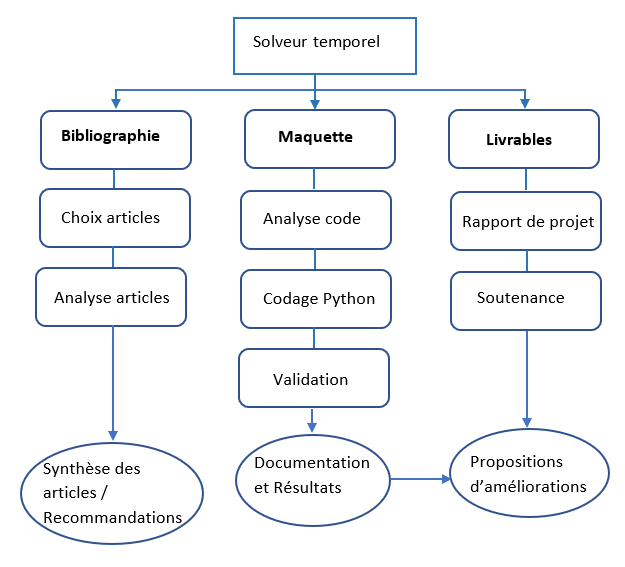
\includegraphics[width=0.7\textwidth]{images/WBS_detaille.PNG}
        \caption{Diagramme PBS}
    \label{PBS}
    \end{figure}
\newpage
    \paragraph{}
    L'utilisation de ces outils nous a permis de délimiter le périmètre de travail afin de rester focalisé sur l'objectif du client et de ne pas divaguer. Ici le diagramme WBS (cf figure \ref{WBS})n'est pas détaillé à son maximum par soucis de lisibilité. Cet outils donne une bonne idée d'ensemble de toutes les tâches qui sont a réalisées dans un ordre précis pour aboutir au résultat final du projet. 
    \begin{figure}[h!]
        \centering
        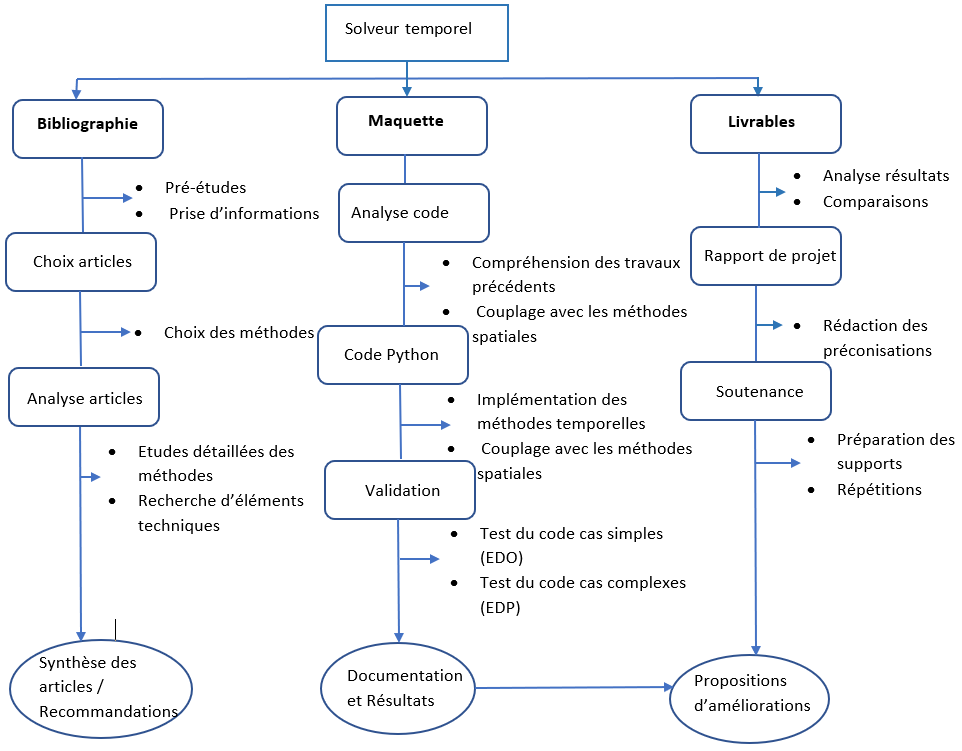
\includegraphics[width=1\textwidth]{images/Vrai_WBS.PNG}
        \caption{Diagramme WBS}
        \label{WBS}
    \end{figure}
\newpage 
    \subsubsection{Organisation de l'équipe}
    \paragraph{}
    La répartition du travail c'est faite assez naturellement en deux équipes grâce aux diagramme PBS et WBS vu précédemment. Nous connaissions très bien les limites de notre projet et les étapes à effectuer pour parvenir aux objectifs du client. Chacun a pu trouver sa place au sein de la configuration suivante (cf figure \ref{fig:OBS}):
    \begin{itemize}
        \item Théo Maes est le chef de projet. 
    \end{itemize}
    \paragraph{}
    Nous avons divisé l'équipe en deux groupes opérationnels :
    L'équipe développement, coordonnée par Sara Barrasa-Ramos, sera responsable de l'implémentation des méthodes numériques. Elle sera composée de :
   	    \begin{itemize}
   	    \item Louis Reboul
   	    \item Sara Barrasa-Ramos
   	    \item Théo Maes
    \end{itemize}
    \paragraph{}
    L'équipe couplage, coordonnée par Pierre Seize, sera responsable de rendre compatible les schémas numériques d'intégration temporelle avec les schémas numériques d'intégration spatial existants. Elle sera composée de :
   \begin{itemize}
        \item Pierre Seize
   	    \item Jean-Baptiste Fourtout
    \end{itemize}
   \paragraph{}
   Cette répartition ayant été faite en consensus avec l'ensemble de l'équipe, en prenant en compte les préférences de chacun et le niveau de connaissance dans ce domaine d'application des sciences. Nous nous sommes efforcés de conserver le plus possible cette répartition du travail.  Néanmoins nous avons été contraints d'effectuer certains changements temporaires de ressources humaines au cours du projet pour palier a des problématiques qui seront expliquées plus en détail par la suite.
    \begin{figure}[h]
    \centering
        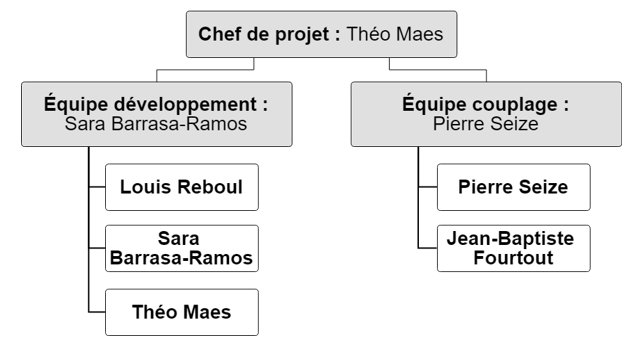
\includegraphics[scale=0.7]{images/OBS.png}
      	\caption{Organisation de l'équipe} 
   \label{fig:OBS}
    \end{figure}

    \subsubsection{Organisation du travail}
    \paragraph{}
    Il nous semble important d'aborder la matrice RACI qui est née de l'association des diagrammes OBS et WBS. En effet, cette matrice permet de repérer le rôle de chacun des membres de l'équipe pour une tâche donnée comme il est indiqué figure \ref{fig:RACI}.
    \paragraph{}
    La lettre R signifie "Réalisation" dans le sens ou les personnes assujettis à cette lettre pour une tâche leur indique qu'ils doivent fournir un travail. Ce qui est différent si la personne est associée à la lettre C signifiant "Consultation". Car c'est simplement qu'elle peut posséder des connaissances, un point de vue intéressant sur la réalisation de la tâche. Cette consultation est effectuée en amont de la réalisation contrairement à l'indice I pour "Information" qui sont des conseils promulguer par des gens qui ont la connaissance pour améliorer la réalisation de la tâche. Et enfin le caractère A signifie "Approbation" ce sont les personnes qui vont prendre les décisions. Dans le cadre de notre petit projet scolaire cela se restreint à notre chef de projet, de manière générale.\\
    Il est évident que le chef de projet ne sert pas qu'à l'approbation des tâches réalisées par ces camarades il participe au même titre que tout le monde.
    \begin{figure}[h]
        \centering
        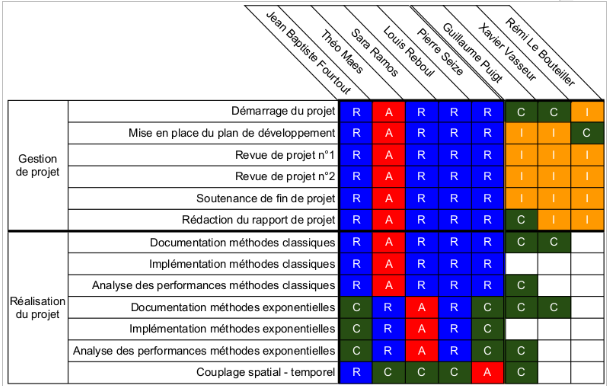
\includegraphics[width=\textwidth]{images/OB2.png}
  	    \caption{Matrice RACI} 
    \label{fig:RACI}
    \end{figure}
    \paragraph{}
    Cette matrice est intéressante car elle permet à chacun des collaborateurs de voir avec qui il travaille sur une même tâche et de pouvoir échanger avec eux. On identifie d'autant plus rapidement les personnes "expertes" qui sauront nous orienter dans le cas d'un blocage lors de la réalisation d'une tâche. 
 
\newpage    
\subsection{Processus du développement}
    
    \subsubsection{Logique de développement}
    \paragraph{}
    Notre logique de développement du projet s'articule principalement sur les différents groupes de tâches qui ont été répertoriés dès la mise en place du projet à l'aide des diagramme PBS et WBS.
    \paragraph{}
    En toute logique nous avons commencé par prendre connaissance de la bibliographie qui est directement fournie par notre client. Puis il a fallu prendre en main la programmation avec le langage Python car tous les développeurs n'avaient pas la même connaissance de ce langage informatique.
    \paragraph{}
    Une analyse approfondie des articles scientifiques et des recherches personnelles du groupe ont permis à l'équipe développement de faire un choix sur les méthodes temporelles qui seront étudiées plus en profondeur. C'est sur des conseils et en accord avec notre client que nous avons fait ces choix. En parallèle l'équipe se chargeant du couplage spatial-temporel devait comprendre en profondeur le fonctionnement du code informatique fournit pour établir une stratégie pour pouvoir y adapter le travail de l'équipe développement.
    \paragraph{}
    Puis logiquement nous avons implémenté les nouvelles méthodes de résolution temporelle dite "Exponentielle", pendant que l'équipe couplage testait le couplage spatial-temporel avec les méthodes usuelles que l'équipe développement a mis très rapidement en oeuvre au début du projet.
    \paragraph{}
    Une fois que l'équipe développement eut réussi à implémenter une méthode exponentielle, l'équipe couplage pu lancer une phase de test pour vérifier le bon fonctionnement du couplage des méthodes sur des cas simples puis plus compliqués.
    
    \subsubsection{Définition des jalons}
    \paragraph{}
    Définition des jalons et la nature des jalons :
    \begin{itemize}
       	\item 21/11/2018 : Première revue de projet à Présentation orale de l'avancée des travaux
       	\item 30/01/2018 : Deuxième revue de projet à Présentation orale de l'avancée des travaux plus début de rapport du projet
       	\item  Mi-Mars : Soutenance de projet à Présentation orale de l'ensemble du projet et des problèmes rencontrés
       	\item  Fin Mars : Livraison des livrables à Rapport de projet, Code source
    \end{itemize}
    \paragraph{}
    Les jalons étant fixés dans la plupart du temps dès le début du projet ils permettent de donner un "tempo" au travail a effectuer. En complément avec le diagramme WBS, et les coûts associés à chaque tâche on permit de rapidement établir un premier diagramme de Gantt (cf figure \ref{fig:Gantt_initial}).

    \subsubsection{Planning de projet}
    \begin{figure}[h]
        \centering
        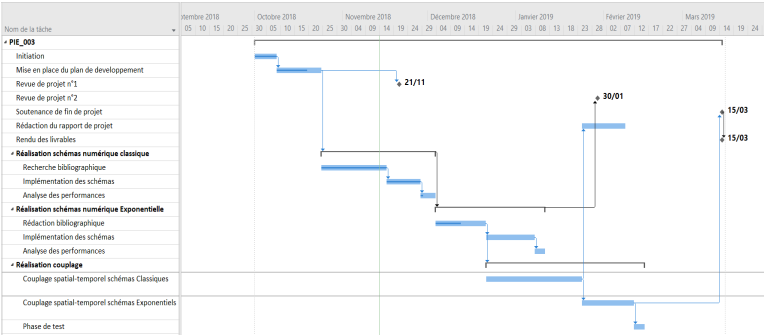
\includegraphics[width=\textwidth, height=8cm]{images/Gant.png}
        \caption{Diagramme de Gantt intial} 
    \label{fig:Gantt_initial}
    \end{figure}
    \paragraph{}
    Après plusieurs entretiens avec le client nous avons convenu de plusieurs changements qui ont provoqués des différences majeures dans l'emploi du temps du projet. 
    \paragraph{}
    Nous nous occupons de la partie intégration temporelle, néanmoins cette partie doit être couplée avec les méthodes d'intégration spatiales. Ces méthodes ont été réalisées au préalable par d'autres groupes d'étudiants de Supaero dans les années antérieures. Pour l'équipe couplage il s'est avéré difficile de reprendre le code informatique tel qu'il nous était fourni pour le coupler avec notre travail sur l'intégration temporelle. Après discussion avec nos clients nous avons donc réussi à les convaincre de changer la structure du code afin que cela soit plus fonctionnelle qu'avant. 
    \paragraph{}
    Cette tâche supplémentaire était un risque très important pour notre projet. Car le code informatique étant fonctionnelle nous pouvions le dégrader et le rendre inutilisable. Pour prévenir de ce risque nous avons donc fait une copie, et modifier seulement la copie. Dans un second temps cette tâche n'était pas prévue à la base dans le diagramme de Gantt initial. Il y avait donc un risque de passer trop de temps sur cette opération et compromettre l'ensemble du projet. 
    \begin{figure}[h]
        \centering
        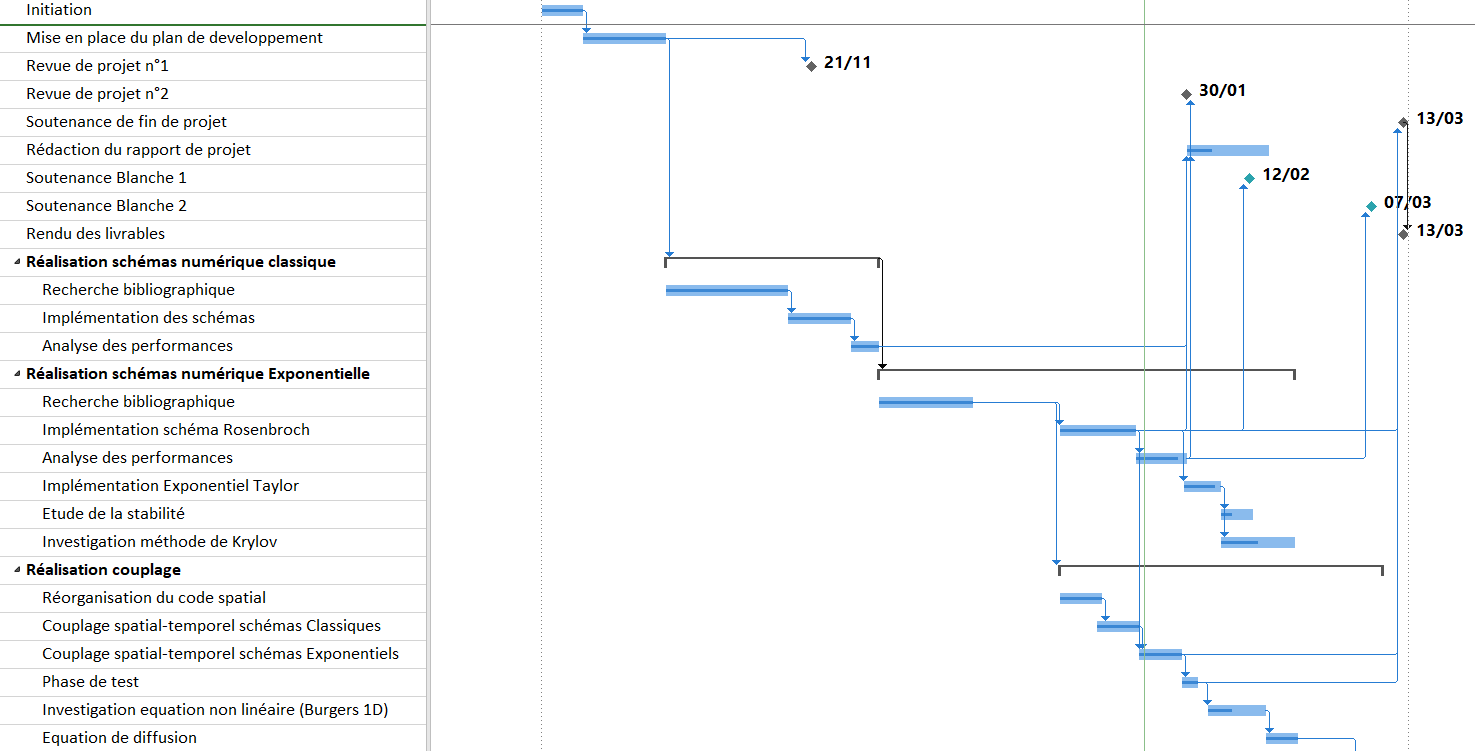
\includegraphics[width=\textwidth, height=8cm]{images/Gantt_revue_2.PNG}
        \caption{Diagramme de Gantt modifié} 
    \label{fig:Gantt modifié}
    \end{figure}
    \paragraph{}
    Finalement comme nous pouvons le voir sur la figure \ref{fig:Gantt modifié} ce risque c'est transformé en opportunité. Car elle a été effectuée rapidement et avec succès ce qui a permit à l'équipe couplage de gagner un temps considérable sur la suite du projet.
    \paragraph{}
    En parallèle l'équipe développement a eu des difficultés sur l'implémentation des schémas temporels. Le travail de l'équipe couplage étant conditionné par la réussite de l'équipe développement nous avons fait le choix de déplacer une ressource humaine dans l'équipe implémentation. Nous avons donc globalement pris de l'avance sur les objectifs initiaux fixés du projet. 
    \paragraph{}
    Le diagramme de Gantt est l'outil principal que nous avons utilisé tout au long du projet. Il permet de situé temporellement parlant le travail effectué par rapport aux prévisions. Ce qui est très utile quand nous avons les demandes du clients qui évoluent au cours du projet.
    \paragraph{}
    Par exemple le client a exigé des soutenances de projet « blanches » mi-février et début mars. Ceci nous a donc imposé donc de préparer des présentations oral supplémentaire et d'arranger le répartition du travail de façon à avoir de nouveaux  résultats à montrer au client lors de la soutenance. Ces aléas d'emploi du temps ont donc été très bien gérer par l'équipe grâce au diagramme de Gantt ces modifications apparaisse en comparant les figures \ref{fig:Gantt_initial} et \ref{fig:Gantt modifié}.


\subsection{Les livrables du projet}
    
    \subsubsection{Liste des produits livrables au client}
    \paragraph{}
    Les livrables du projet :
    \begin{itemize}
       	\item Revue bibliographique avec pour objectif de répondre aux questions qu'est ce qu'on conseil d'utiliser et pourquoi ? Pour quelles applications ?
       	\item Compte rendu de projet sous format papier (ci-présent)
       	\item Rendu des supports utilisés pour la soutenance finale, un fichier Power Point
       	\item  Code informatique avec pour critère d'acceptation d'être fait en langage Python et transmis par la plateforme GitHub.
    \end{itemize}

    \subsubsection{Liste des livrables demandés par le corps enseignant}
    \paragraph{}
    Dans le cadre de la gestion de projet nous devons rendre un plan de développement de notre projet. D'autre part nous sommes évalués sur un rapport de projet et une soutenance qui aura lieu mi-Mars ce sont donc des livrables requis.
    \paragraph{}
    Un dernier livrable requis est une fiche synthèse de taille A4 résumant brièvement les enjeux du projet et les résultats obtenus. 


\subsection{Risques et opportunités}
    \paragraph{}
    Les risques liés au projet sont répertoriés dans le tableau figure \ref{Tab risque}. On peut voir que ce tableau est réalisé en définissant pour chaque risque potentiel une Occurrence et une Gravité par un coefficient. Et le produit de ces deux coefficient nous indiquera tout naturellement si l'impact du risque considérer sur le projet est fort ou non. L'utilisation d'un code couleur permet en effet de visuellement repérer les risques majeurs d'un coup d'oeil avec la couleur rouge.
    \paragraph{}
    Une fois ces risques identifiés il est à notre charge de faire en sorte qu'ils ne se produisent pas. C'est donc ce que nous nous sommes efforcés de faire tout au long du projet. Bien sûr ayant une faible expérience des projets il est difficile d'identifier en amont tous les risques qu'un projet peu contenir.
    \paragraph{}
    Il y a d'ailleurs un risque que nous n'avions pas considéré c'est incompatibilité ou la difficulté de couplage de notre travail avec la méthode spatiale. En effet, la méthode spatiale étant fournit par le client nous récupérions un code informatique fonctionnant. Néanmoins il était codé de manière peu flexible ce qui ne permettait pas de coupler les deux travaux de façon simple et agile.
    \paragraph{}
    C'est alors qu'un choix s'offrait à nous, soit on prenait le temps de réécrire la partie du code fournit par le client soit nous allions avoir des difficultés pour tester les résultats de notre travail et cela allait nous prendre beaucoup de temps. Mais nous aurions la garantit d'avoir un résultat. Ce n'est cependant pas le choix que nous avons fait. Nous avons préférer avec l'accord du client reprendre la structure du code fournit afin de pouvoir faire un couplage de notre travail de manière simple et agile.
    \paragraph{}
    Ce qui s'apparentait à un risque s'est transformé en opportunité car finalement par rapport au diagramme de Gantt initial nous avions gagné du temps. Ce qui nous as permit de faire pas mal de choses supplémentaires par la suite.
    \begin{figure}[h] 
        \centering
        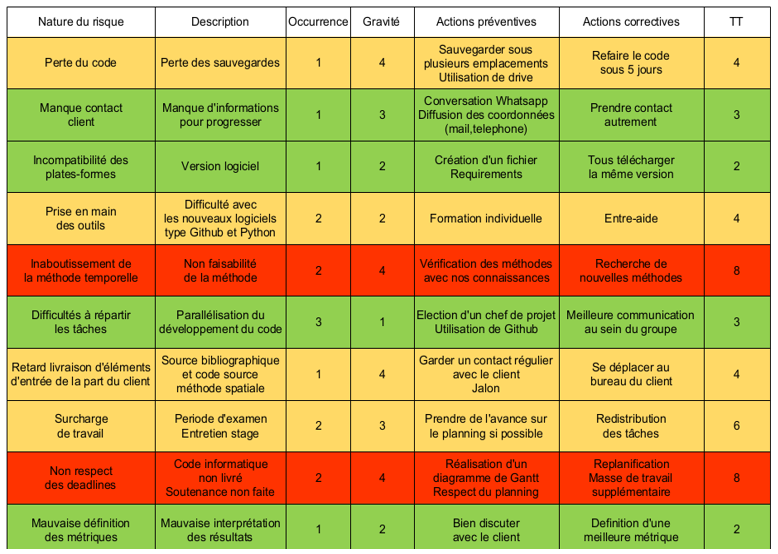
\includegraphics[width=\textwidth]{images/matrice.png}
        \caption{Tableau des risques}
    \label{Tab risque}
    \end{figure}

\subsection{Suivi et Contrôle}
    \subsubsection{Tableau de bord de suivi}
    \paragraph{}
    Nous avons l'opportunité d'utiliser MS-Project pour faire un suivi du projet. Nous avons réalisé un diagramme de Gantt de référence que nous avons mis à jour au fur et à mesure que le projet avançait. Cela nous a été très utile car comme nous l'avons vu précédemment nous avons su réagir vite à des problèmes rencontrés lors du projet. 
    \paragraph{}
    Avec l'élaboration du WBS nous avions pu mettre un coût sur chaque tâche à réaliser et le diagramme de Gantt à mis en évidence qu'en fin de projet des personnes serait en surcharge de travail. Nous nous sommes donc efforcé dès le début du projet à ré-agencer les tâches, mais les aléas du projet nous ont aussi aidé à résoudre ce problème.  
    \paragraph{}
    L'utilisation de la plate-forme GitHub, gérant le versionnage des fichiers possède certaines fonctions aidant aussi à la gestion du projet. On peut voir qui travail sur quoi quasiment en temps réel.
    Pour le partage de documents nous nous sommes créer un groupe sur un site web qui permet le partage et la modification avec plusieurs utilisateurs facilement.
    \paragraph{}
    Ce sont autant de plate-formes qui permettent de garder l'ensemble de l'équipe en contact. Cela à aussi tendance à créer une émulsion et une dynamique de groupe. Néanmoins il faut veiller à ne pas avoir trop d'outils pour ne pas se perdre. Mais dans notre cas chacune des interfaces avait une fonction différentes et bien définie

    \subsubsection{Communication}
    \paragraph{}
    De façon à être dynamique au sein du groupe nous avons mis en place une conversation WhatsApp. Car l'interface utilisée pour cette application est le téléphone, cela permet rapidement d'échanger des informations ou de se donner rendez-vous pour travailler. Un de nos clients est sur cette conversation ce qui lui permet de rester en permanence au courant de l'avancée de notre travail.
    \paragraph{}
    Néanmoins d'un point de vue plus formel il nous paraissait très important d'utiliser les mails, de plus c'était le seul moyen de communication avec certaines parties prenantes du projet.
    \paragraph{}
    D'autre part en moyenne nous avions décidé de faire des réunions bimensuelles dès le début du projet. Sur l'ensemble du projet c'est une contrainte que nous nous sommes imposés mais qui fût respectée et nous a permit de rester à l'écoute de nos clients concernant leurs exigences qui ont évoluées au cours du temps.